\chapter{Modelling for Public Health Intervention}

\section{A Systems Dynamics Model}
A systems model was created using \url{insightmaker.com} to simulate the dynamics of temperature stress mortality in a warmer future West Dorset in 2044 (see Chapter on~\nameref{section:modelstory}). The model was developed with two objectives in mind:
\begin{itemize}
\item To engage policy makers in a discussion about the potential health impacts of climate change on the health of our ageing population.
\item To explore whether interactive systems models and associated story telling is a potentially effective tool in the policy development process and worth exploring further.
\end{itemize}

\subsection{How to use the model}
Follow this link: \href{https://insightmaker.com/insight/33655/Temperature-Stress-Mortality-Simulator}{Temperature Stress Mortality Simulator}\sidenote{insightmaker.com/insight/33655/ Temperature-Stress-Mortality-Simulator} to get the `guest login' that allows participants to change variables, simulation settings and run the simulation (Figure~\ref{fig:IMGuest}). The model starts in `story mode', which allows users to familiarise themselves with the model through a structured story using the `Step Forward' button located in the bottom-right corner of the screen.

There are four menu tabs along the top of the screen: Settings, Simulate, Tools, and Zoom, whose function will be obvious upon exploration. The best place to start -- click on the `Simulate' tab and explore the model output.

The model variables are provided along the right-hand-side of the screen and can be scrolled through to review and each variable can be set with easy to use `slider bars'.
\begin{description}
\item [Age Groups] Choose the age groups or everyone over 70 years (All)
\item [Sex] Older men have a significantly higher base mortality rate
\item [SEC] Socio-economic class has a significant impact on base mortality rates and on simulation results
\item [Reach] Defining the public health intervention
\item [Efficacy] Defining the public health intervention
\item [Intervention Target] Define the thermal stress in which to intervene
\item [Compliance] Defining the public health intervention
\end{description}

Folders, box elements with a `+' in the top-left corner contain further information and model parameters. 

Further information about any element in the model can be had by a left-mouse click on that element. The additional information will be presented on the right-hand side of the screen, and at the bottom of this panel, users can explore systems thinking concepts represented by the element.

Additionally, when you move the pointer over an element an `i' and a `folder' symbol will appear and each of these will also provide further information about that element.

\begin{figure*}[htbp]
\centering
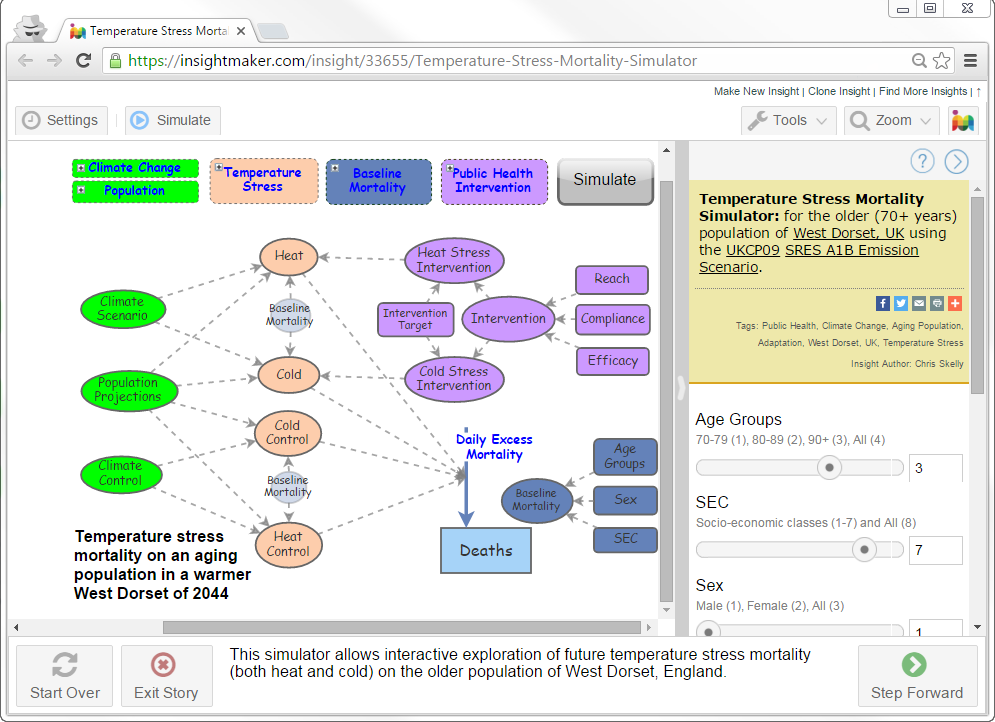
\includegraphics{./CCA/img/InsightMaker_GuestScreen.png}
\caption[Insight Maker Guest Login Screen]{Users of our system model ``Temperature Stress Mortality Simulator'' will be presented with this user interface if they follow the provided link. Note that there are now more menu tabs along the top of the screen: add primitives, flows/transitions/links, edit, style. These tabs contain the tools for editing and creating models.\label{fig:IMGuest}}
\end{figure*}

\subsection{How to modify the model}
Follow this link: \href{https://insightmaker.com/}{Insight Maker}\sidenote{https://insightmaker.com/} to get to the page that allows participants to set up an account, explore other people's models and create your own (Figure~\ref{fig:IMLogin}).

\begin{description}
\item [Create account] `Create a Free Account' -- top-right of screen
\item [Search for Model] `Explore Insights' --> `Find Insights' --> `Search': Temperature Stress Mortality Simulator
\item [Copy Model] Select model --> Clone Insight (top-right menu)\sidenote{You now have your own copy of the model and you can make any modifications to it that you like.}
\end{description}

\begin{figure*}[htbp]
\centering
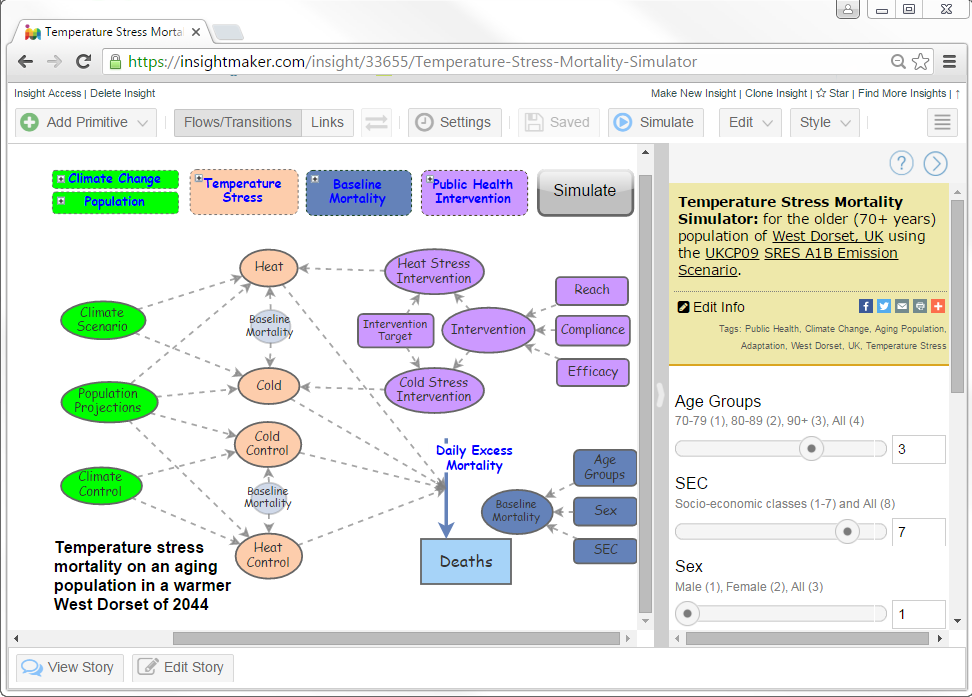
\includegraphics{./CCA/img/InsightMaker_LoggedinScreen.png}
\caption[Insight Maker User Login Screen]{Users of our system model ``Temperature Stress Mortality Simulator'' will be presented with this user interface if they create a free account and make a copy of the model.\label{fig:IMLogin}}
\end{figure*}

\section{Story Telling} \label{section:modelstory}
The `model story' is an interactive tour of the system model developed for this project that was produced using \href{https://insightmaker.com}{Insight Maker}\sidenote{insightmaker.com/}. The story is available online allowing direct interaction with the model \href{https://insightmaker.com/insight/33655/Temperature-Stress-Mortality-Simulator}{Temperature Stress Mortality Simulator}\sidenote{insightmaker.com/insight/33655/ Temperature-Stress-Mortality-Simulator}.

By Chris Skelly\\
June 20, 2015
\begin{description}
	\item[Temperature Stress Mortality Simulator:] for the older (70+ years) population of~\href{http://en.wikipedia.org/wiki/West\_Dorset}{West Dorset, UK}\sidenote{en.wikipedia.org/wiki/West\_Dorset}~using the~\href{http://ukclimateprojections.metoffice.gov.uk/}{UKCP09}\sidenote{ukclimateprojections.metoffice.gov.uk}~\href{http://www.grida.no/publications/other/ipcc\_sr/?src=/climate/ipcc/emission/}{SRES A1B Emission Scenario}\sidenote{www.grida.no/publications/other/ ipcc\_sr/?src=/climate/ipcc/emission/}.
	\item[Acknowledgements] We would like to thank Communities Living Sustainably for funding this project from a Big Lotteries grant and all my colleagues at Dorset Public Health who made this project happen --- Chris Ricketts wrote the proposal and guided its early development, Rebecca Pearce managed the project and Dave Lemon undertook the modelling work to adapt temperature stress to West Dorset.
\end{description}

\begin{figure}[tb]
	\centering
	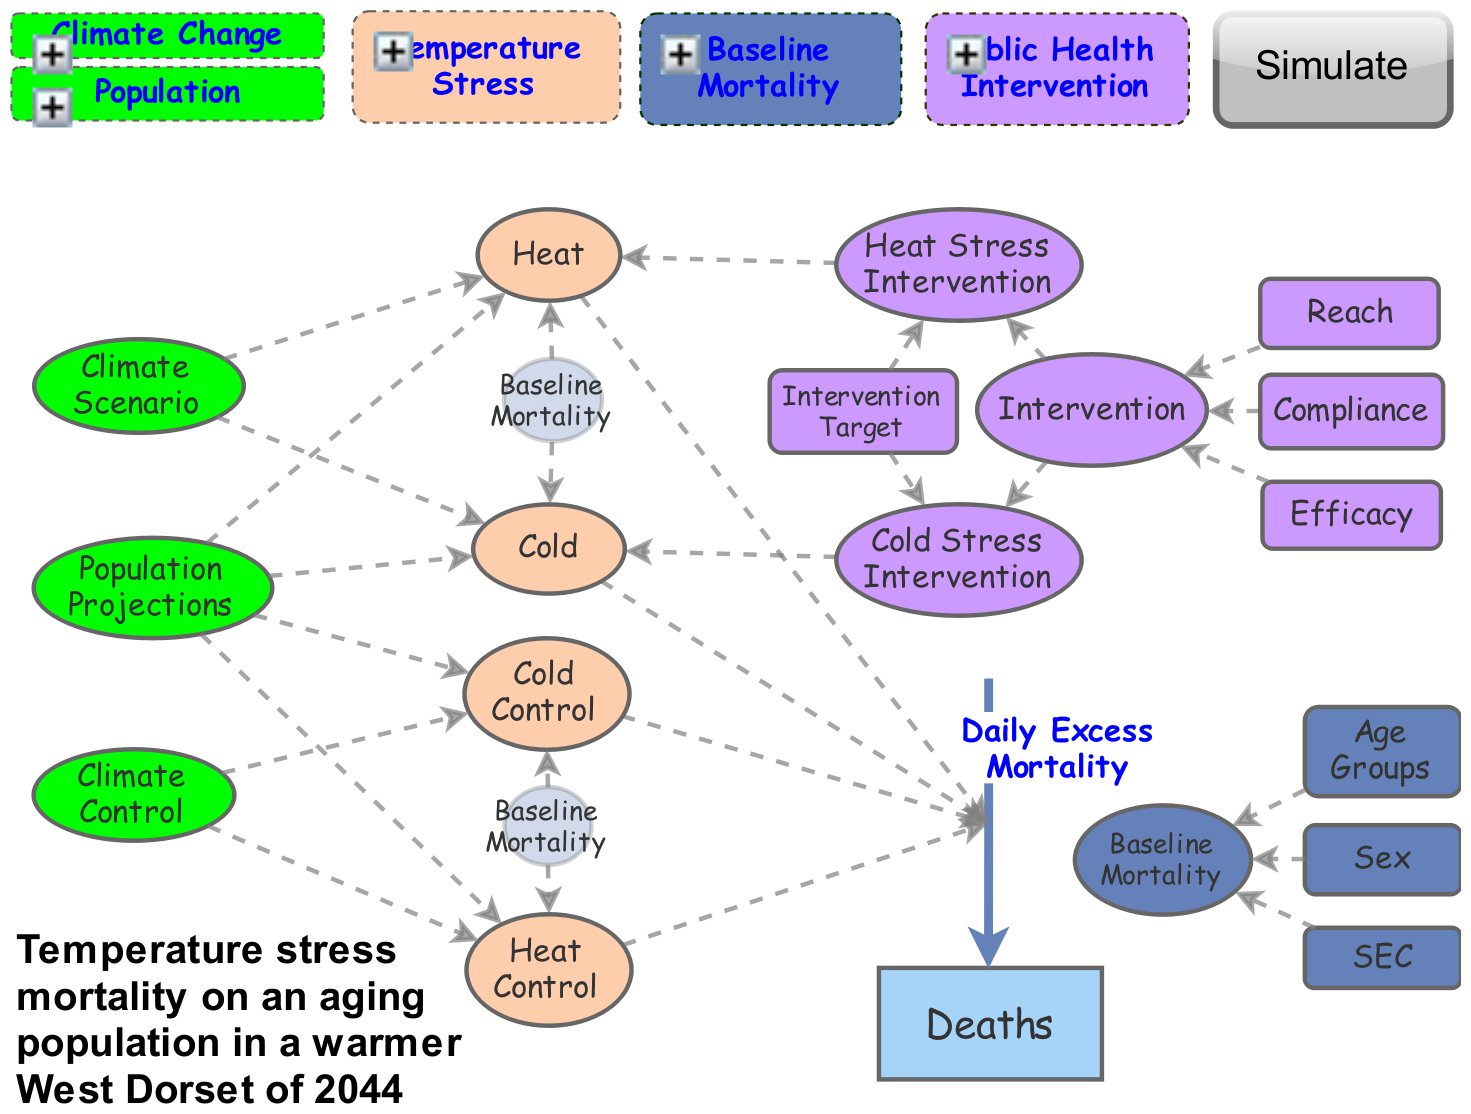
\includegraphics{./CCA/img/image_1.png}
	\caption[System Model Simulator]{This simulator allows interactive exploration of future temperature stress mortality (both heat and cold) on the older population of West Dorset, England.}
\end{figure}

\begin{figure}[htbp]
	\centering
	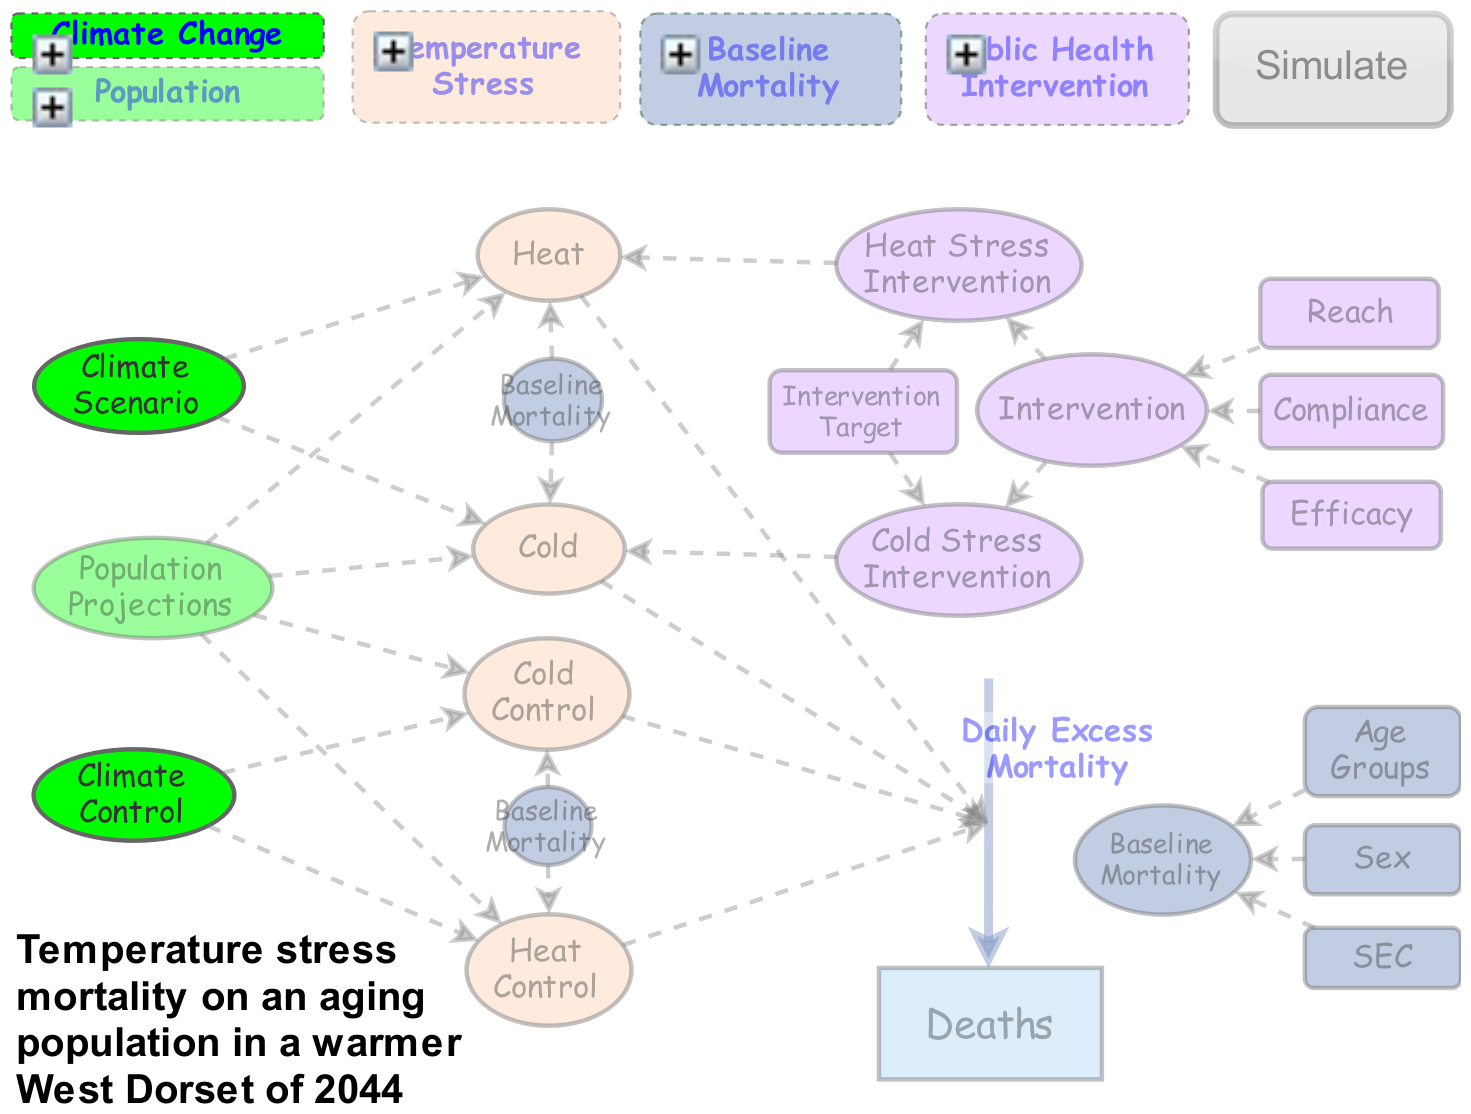
\includegraphics{./CCA/img/image_2.png}
	\caption[UKCP09 Scenario Data]{This simulator is driven using a future climate scenario (UKCP09) that is the basis of much climate adaptation policy in the United Kingdom. It is `downscaled' to the West Dorset region producing plausible daily temperature values for both the climate scenario (2044) and a control period (contemporary observed climate).}
\end{figure}

\begin{figure}[htbp]
	\centering
	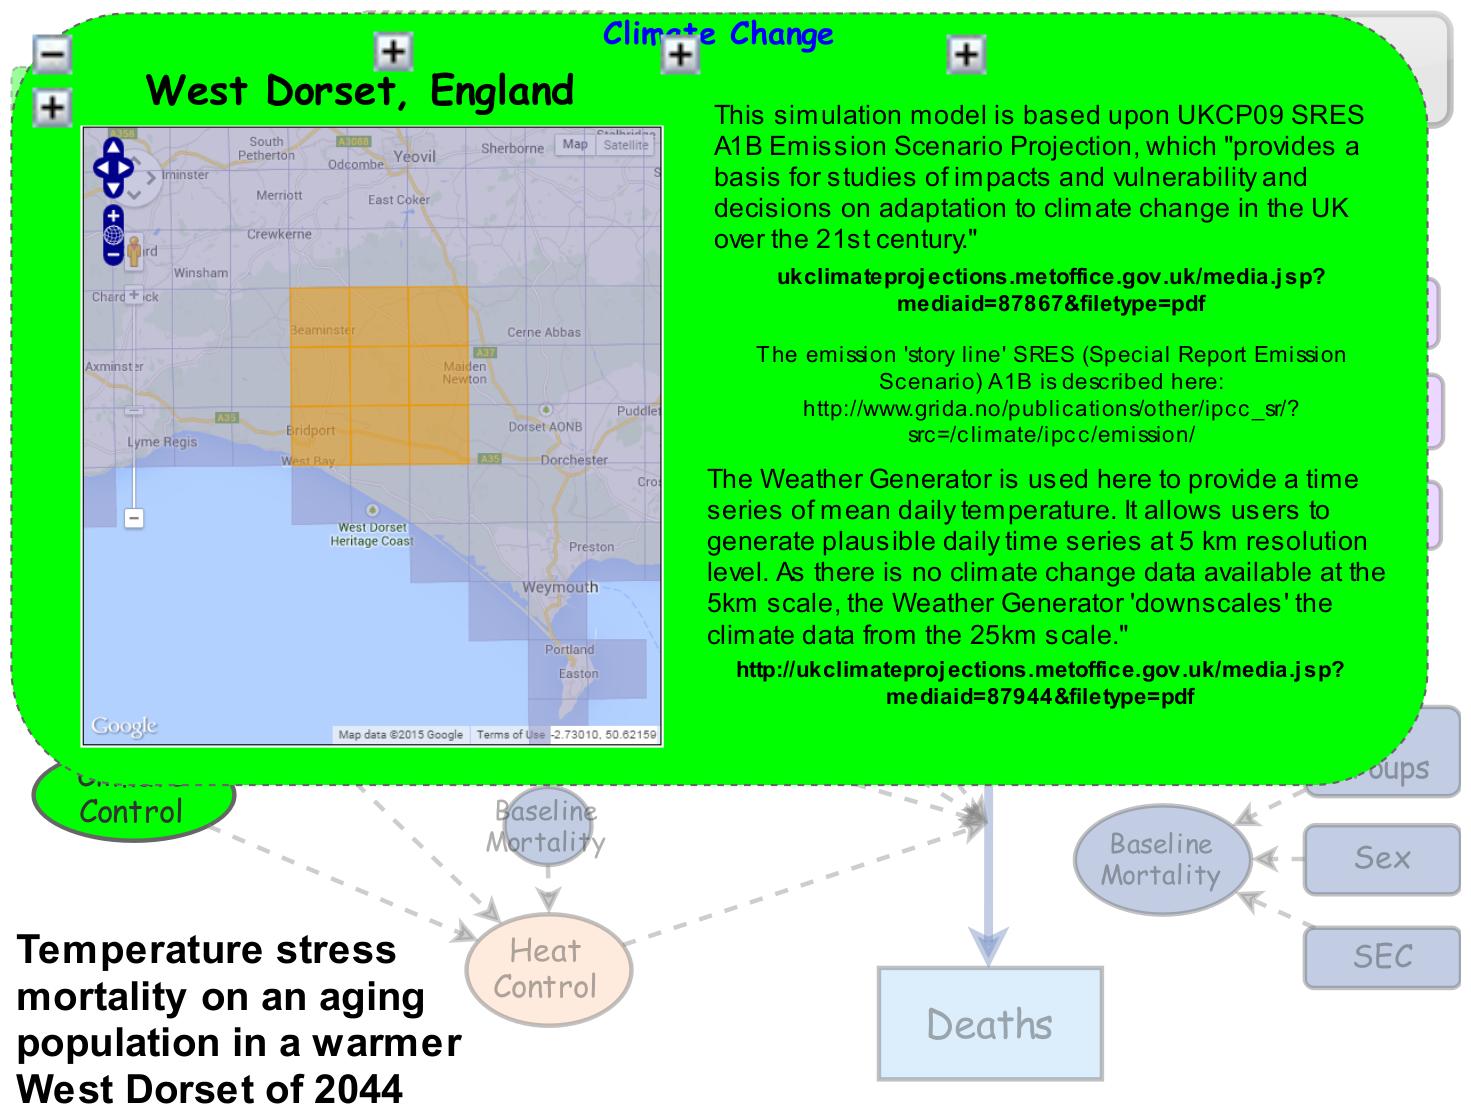
\includegraphics{./CCA/img/image_3.png}
	\caption[Simulated Climate Data]{Simulated climate data and scenarios details are found here.}
\end{figure}

\begin{figure}[htbp]
	\centering
	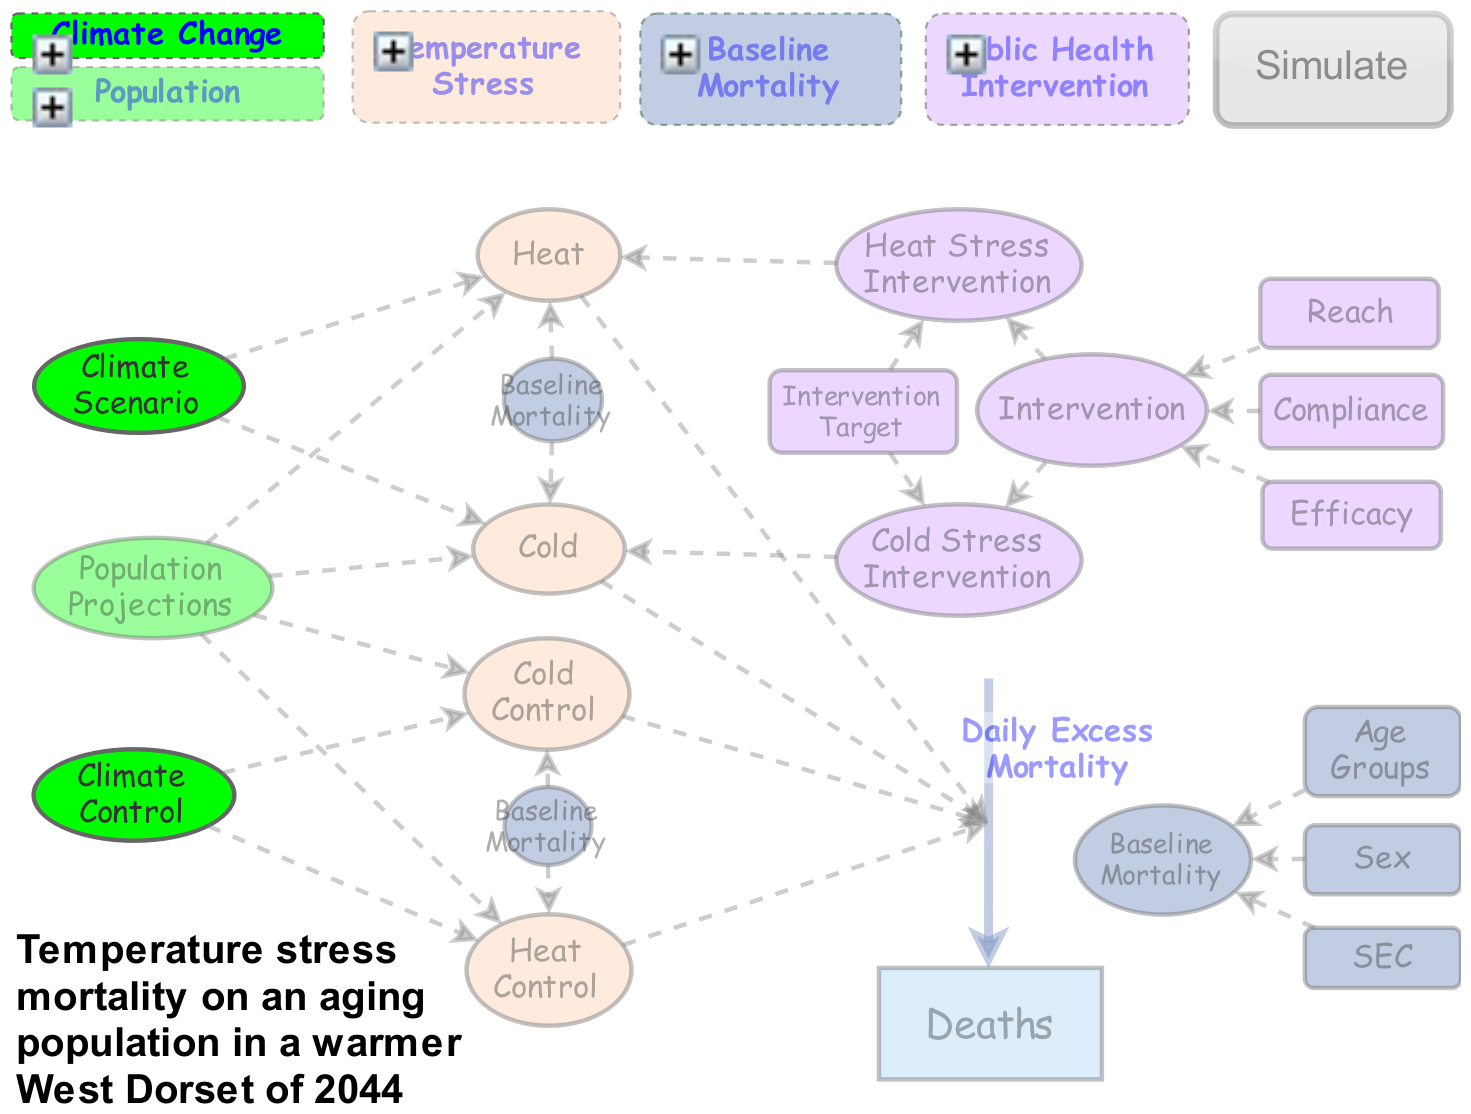
\includegraphics{./CCA/img/image_4.png}
	\caption[Population Change in West Dorset]{The climate is not the only thing that is forecast to change in West Dorset by 2044\ldots}
\end{figure}

\begin{figure}[htbp]
	\centering
	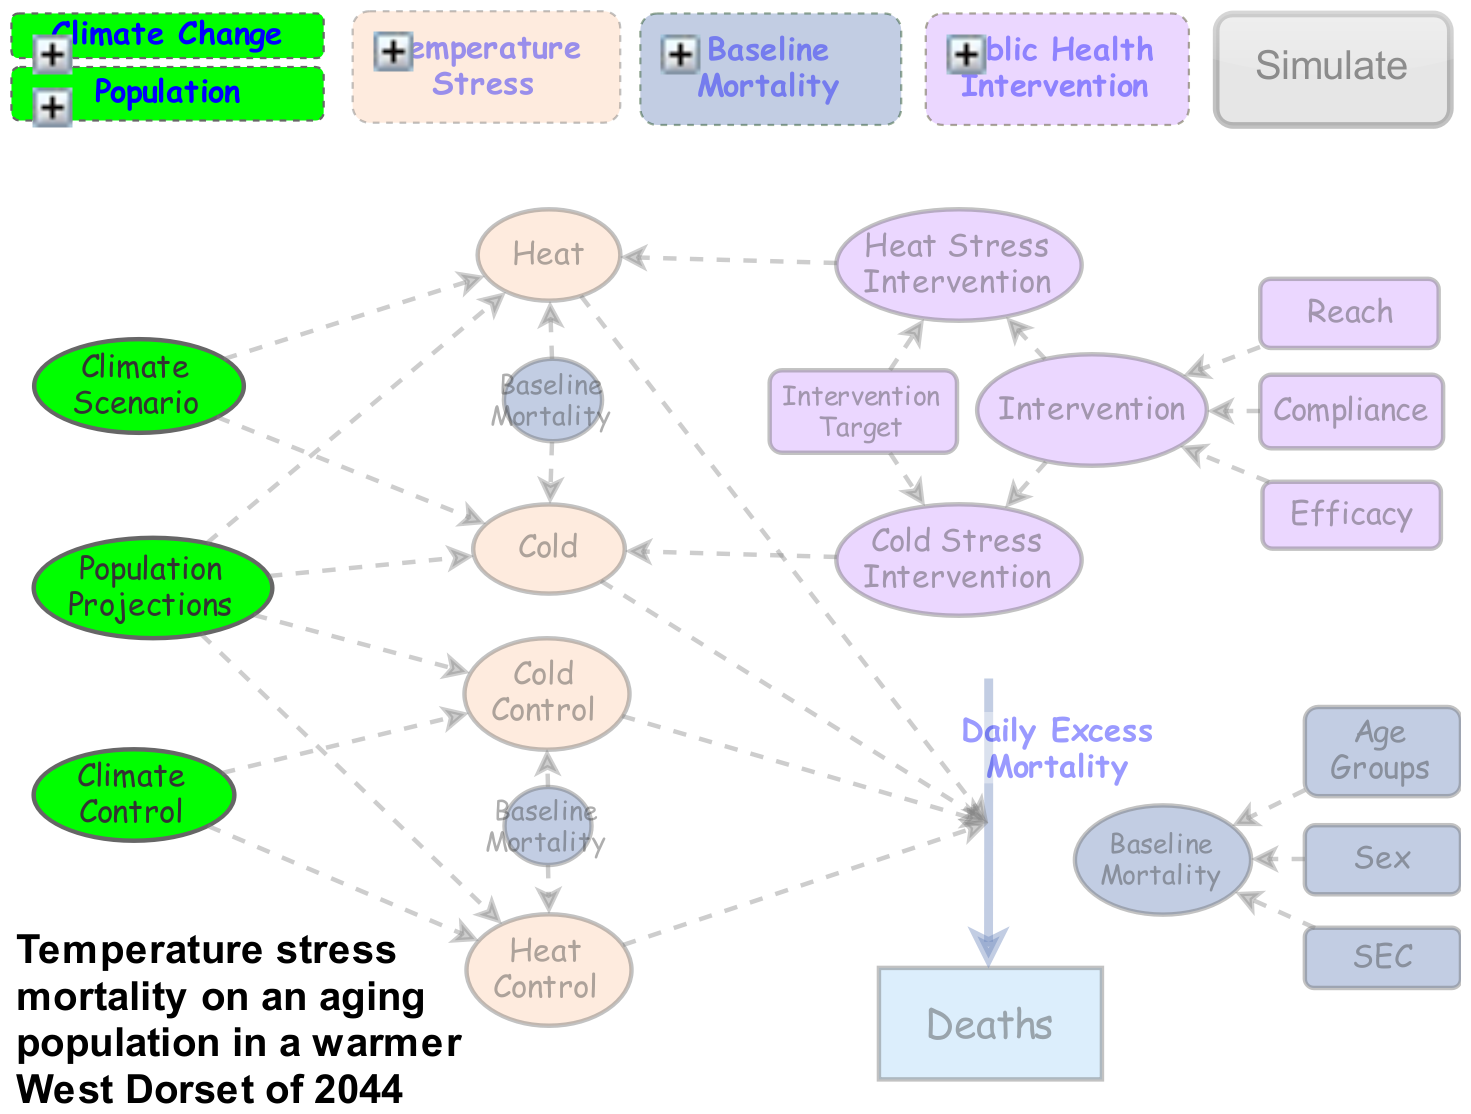
\includegraphics{./CCA/img/image_5.png}
	\caption[Ageing West Dorset Population]{The population of West Dorset, like that of the United Kingdom is ageing. In addition to an ageing population, there has been a retirement migration movement to the Dorset region for many years. This is likely to continue.}
\end{figure}

\begin{figure}[htbp]
	\centering
	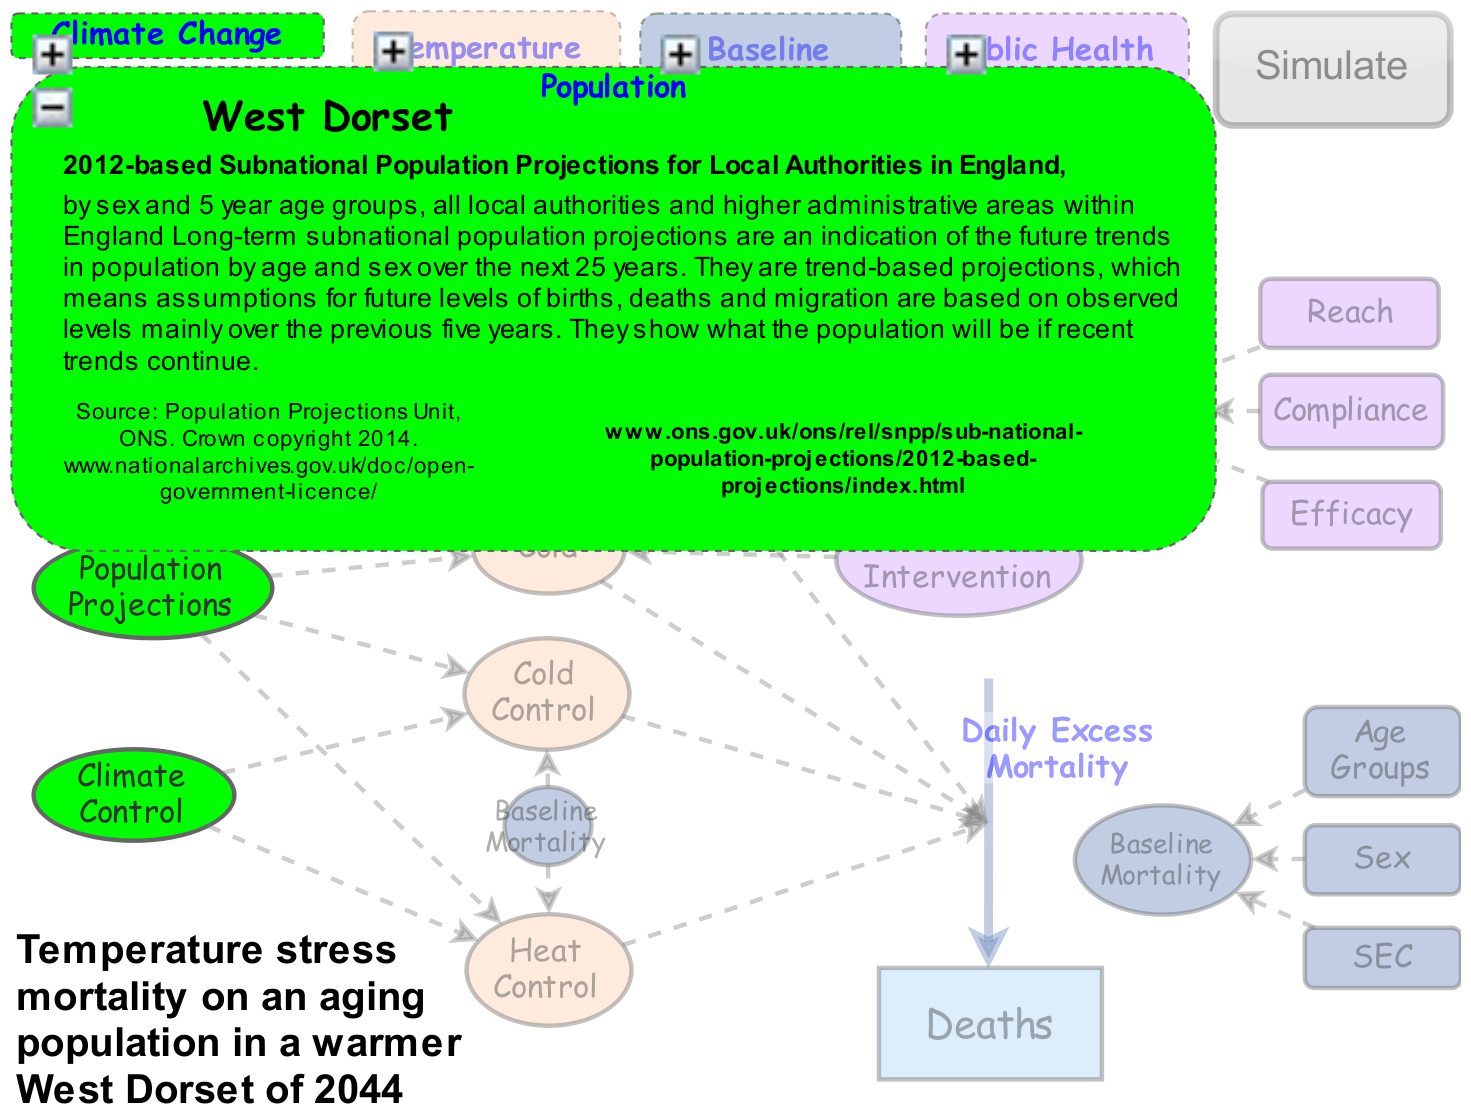
\includegraphics{./CCA/img/image_6.png}
	\caption[ONS Population Projections]{Population projection data, from the~Office of National Statistics, is detailed in this folder.}
\end{figure}

\begin{figure}[htbp]
	\centering
	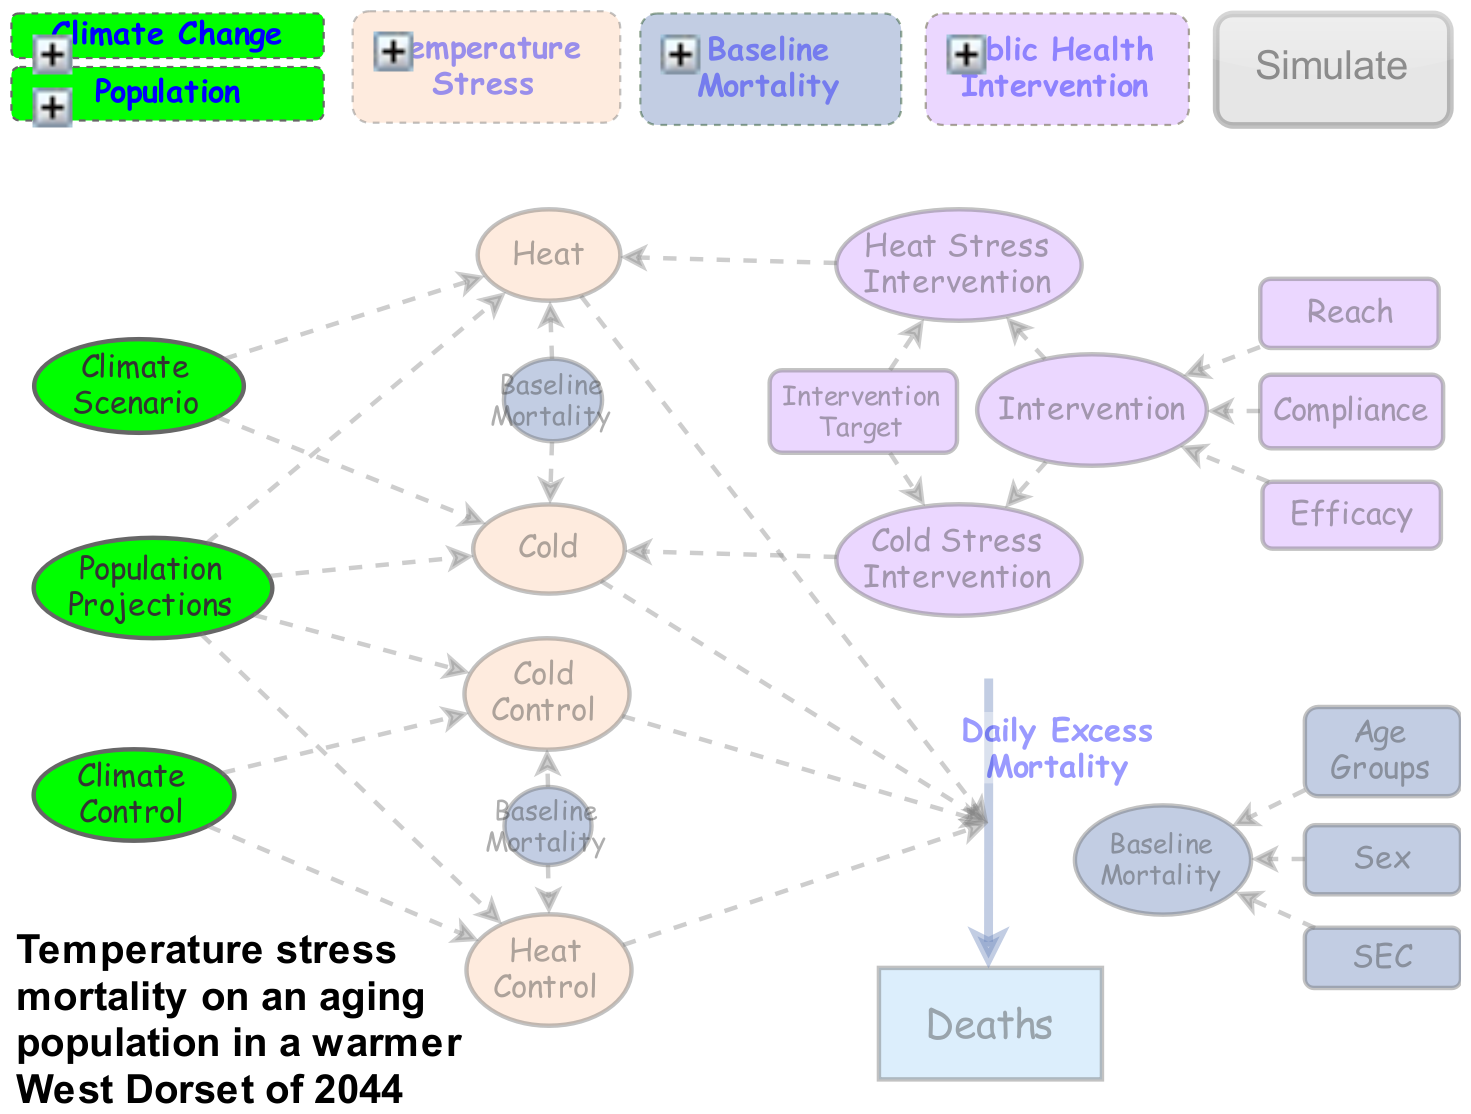
\includegraphics{./CCA/img/image_7.png}
	\caption[Climate Warming and Population Ageing]{The climate is expected to warm and the population is expected to age.}
\end{figure}

\begin{figure}[htbp]
	\centering
	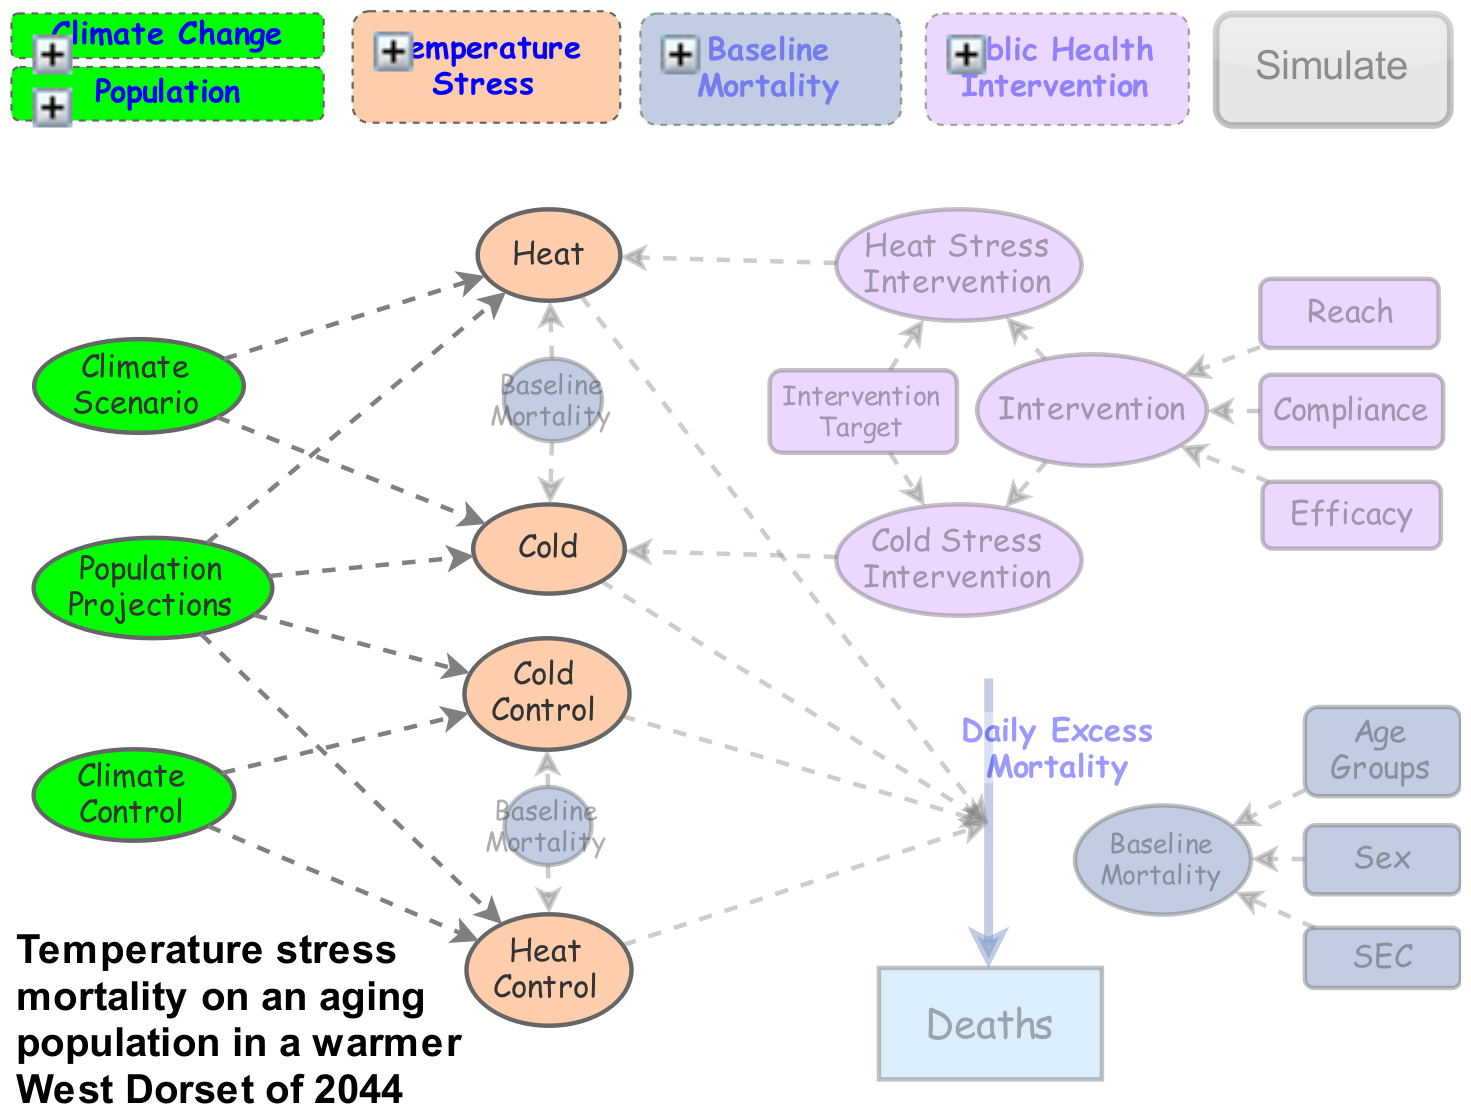
\includegraphics{./CCA/img/image_8.png}
	\caption[Thermal Stress]{Human physiology responds to ambient temperatures. If it is too warm or too cold the human body is stressed. This is most noticeable during major heatwaves when most of the population can feel the `heat stress'.}
\end{figure}

\begin{figure}[htbp]
	\centering
	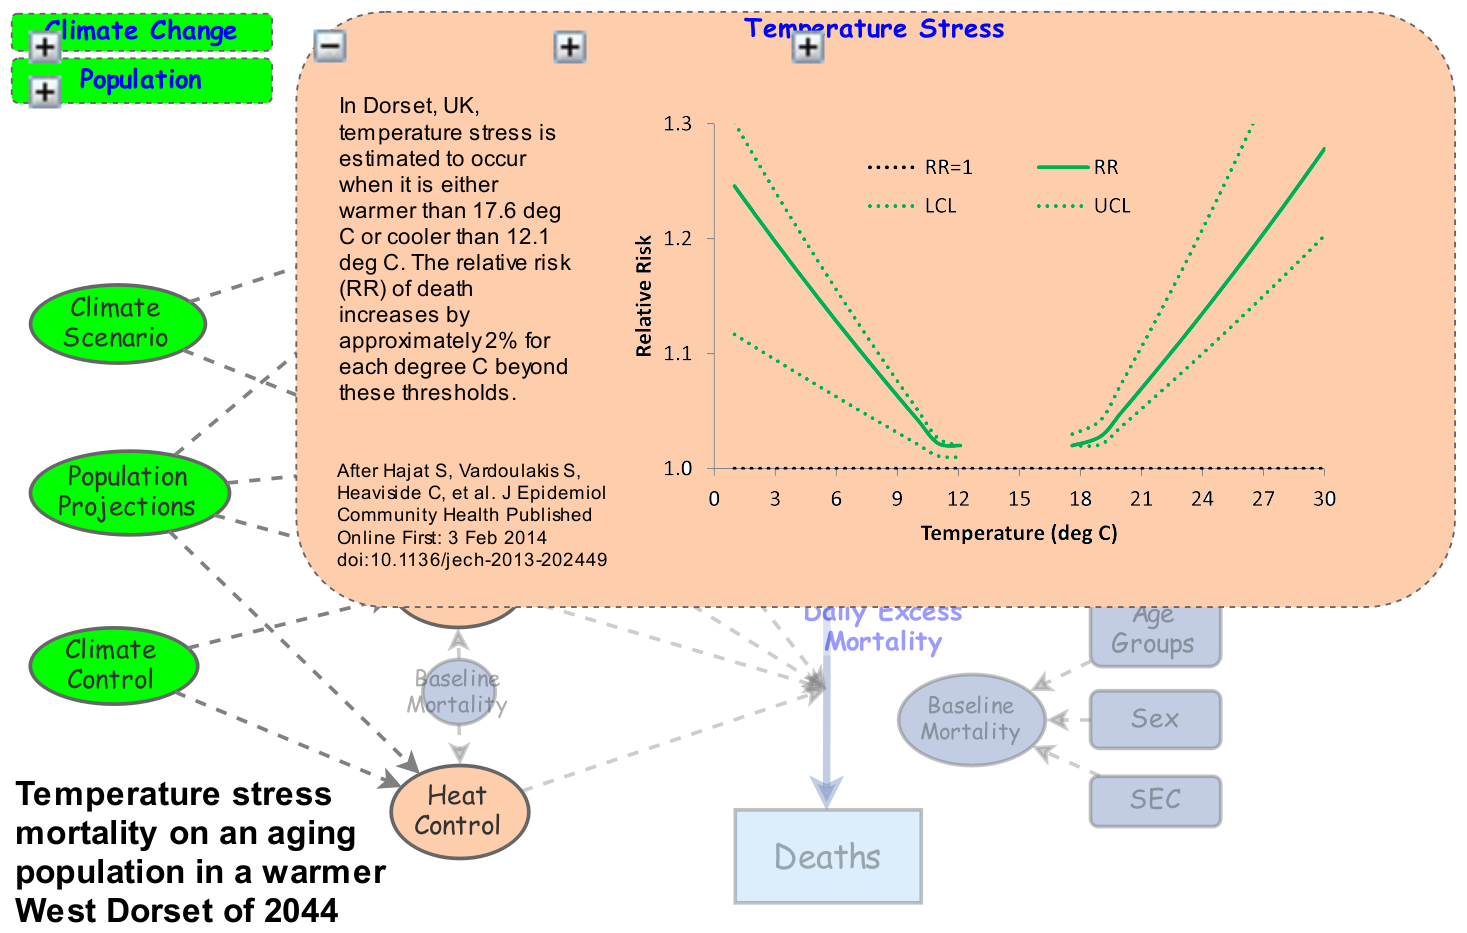
\includegraphics{./CCA/img/image_9.png}
	\caption[Thermal Stress Thresholds]{However, temperature stress occurs far more frequently than we might think -- and in Dorset at almost any time of year. Additionally, as we age, we tend to `feel' the cold or heat more. In other words, we experience more temperature stress. We have adapted a model that estimates the mortality associated with temperature stress in the West Dorset climate. It uses a `base mortality rate' (more on this later) for a population to estimate the temperature stress related `excess mortality'. This model shows that for every 1 degree C in temperature over either a heat or cold threshold excess mortality increases by 2\%. This is the fundamental relationship upon which this simulator is based.}
\end{figure}

\begin{figure}[htbp]
	\centering
	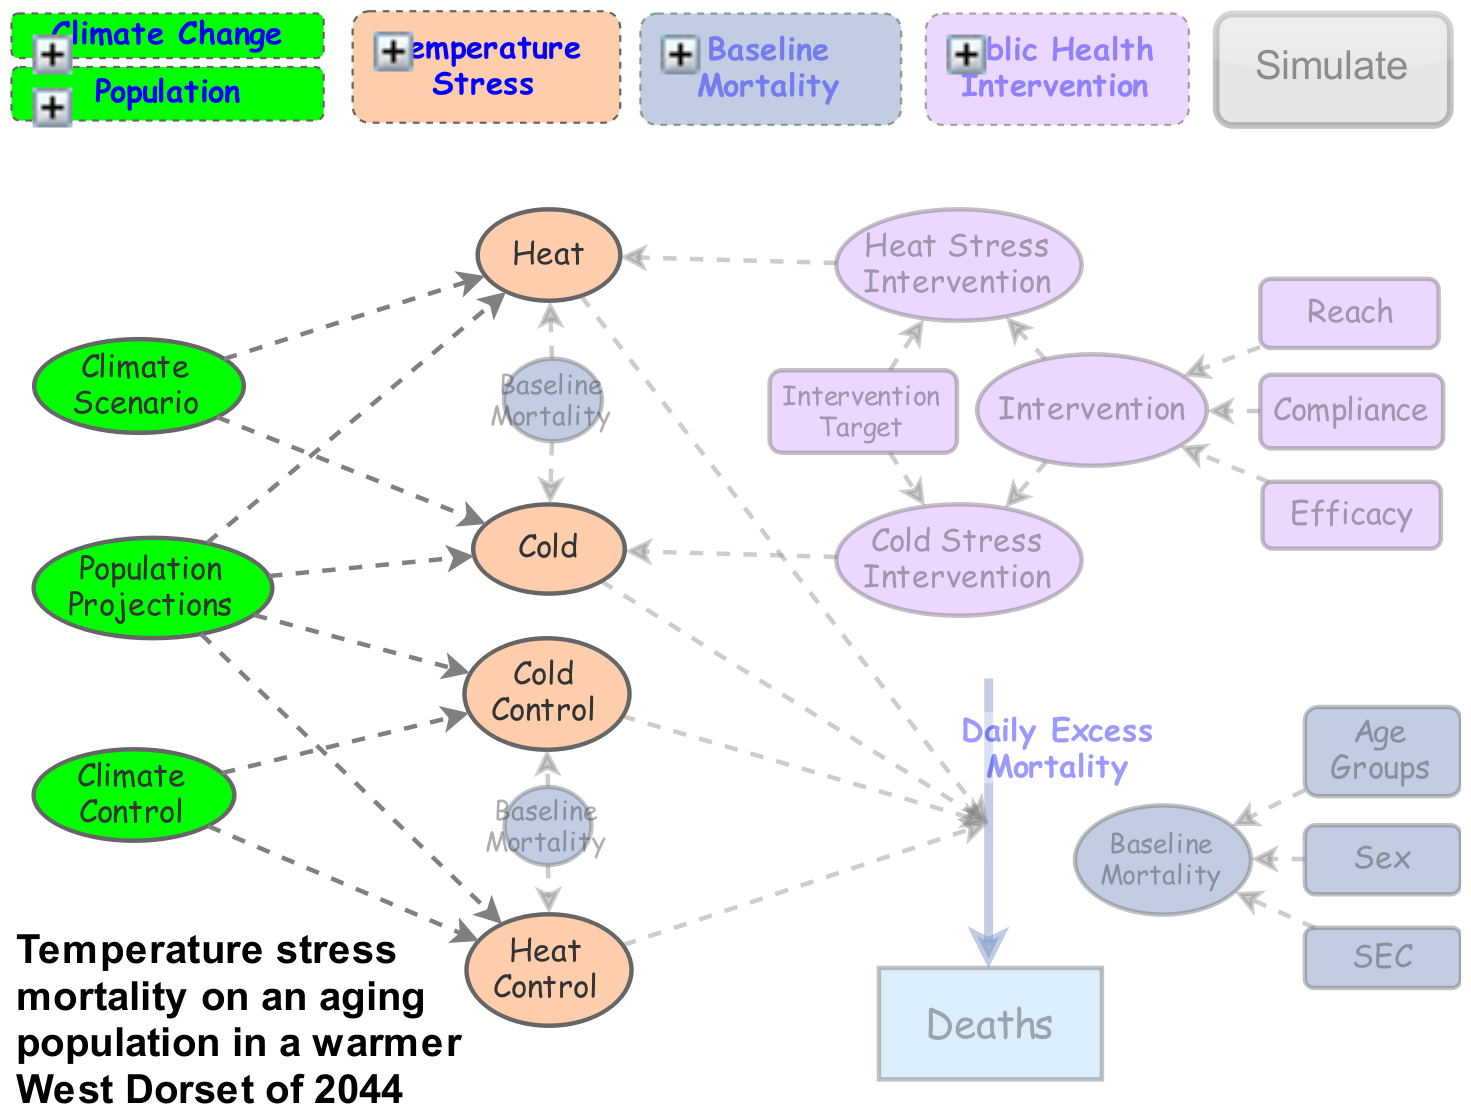
\includegraphics{./CCA/img/image_10.png}
	\caption[Base Mortality Rates]{The relationship between temperature and the base mortality rate is how we define `temperature stress'. But where do these `base mortality rates' come from?}
\end{figure}

\begin{figure}[htbp]
	\centering
	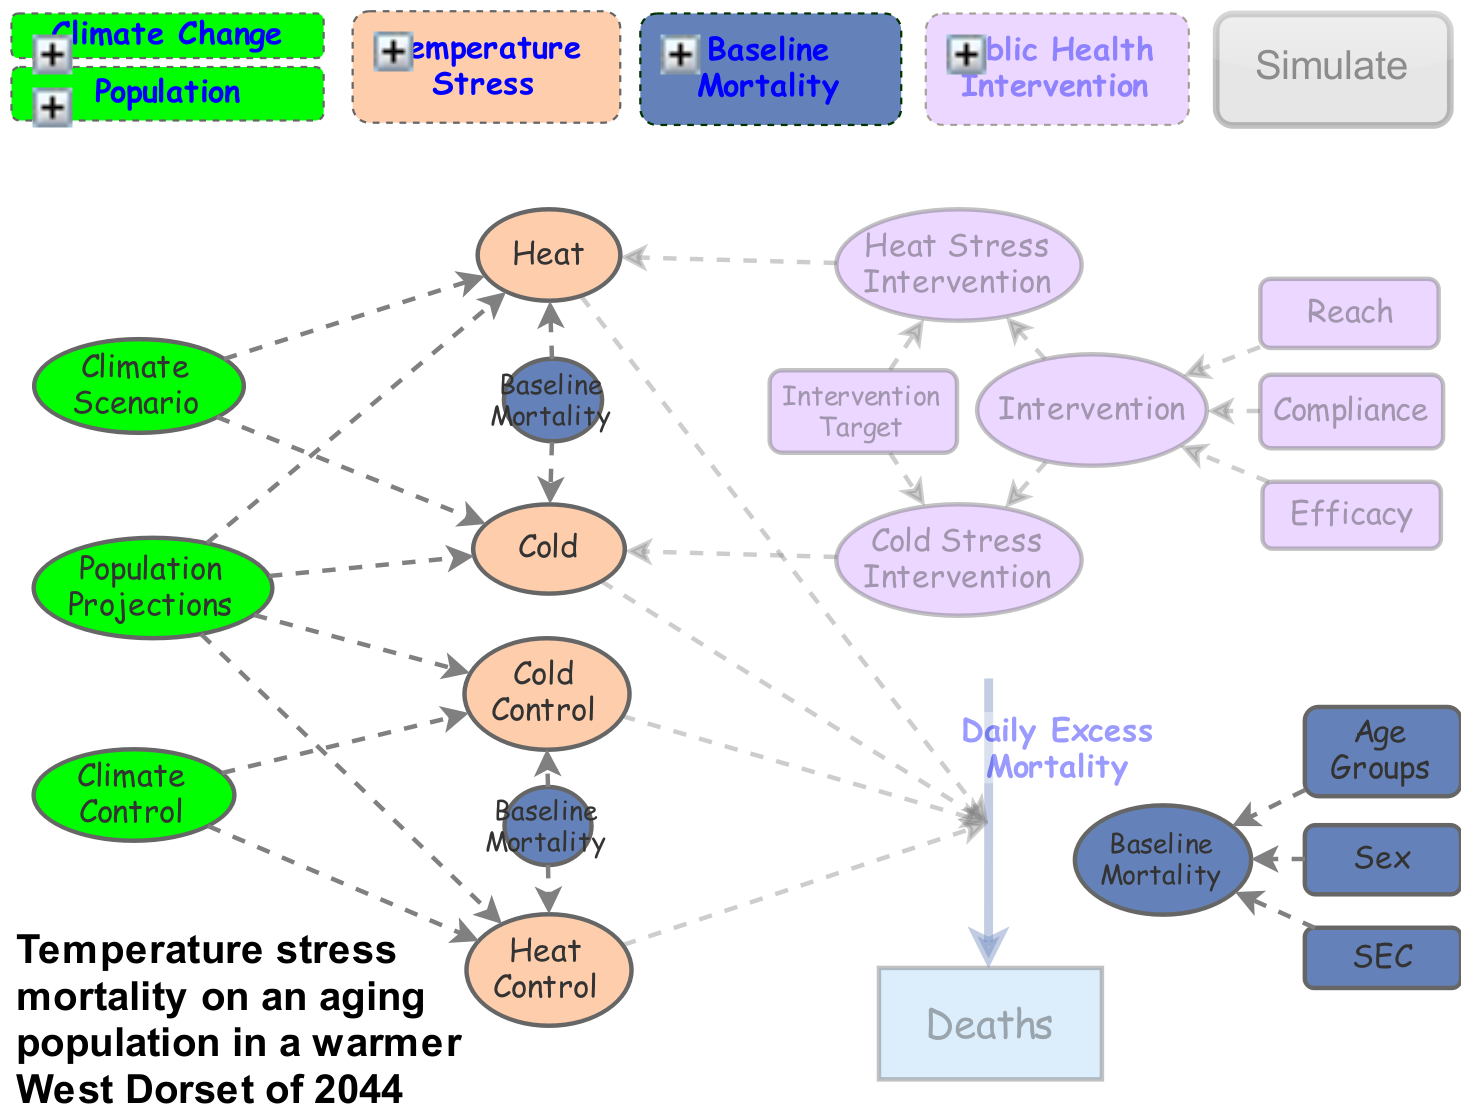
\includegraphics{./CCA/img/image_11.png}
	\caption[Age Specific Base Mortality Rates]{Base mortality rates are produced in the United kingdom for different groups by age, gender and socio-economic class (SEC), because it is well established that there are significant inequalities across these groups.}
\end{figure}

\begin{figure}[htbp]
	\centering
	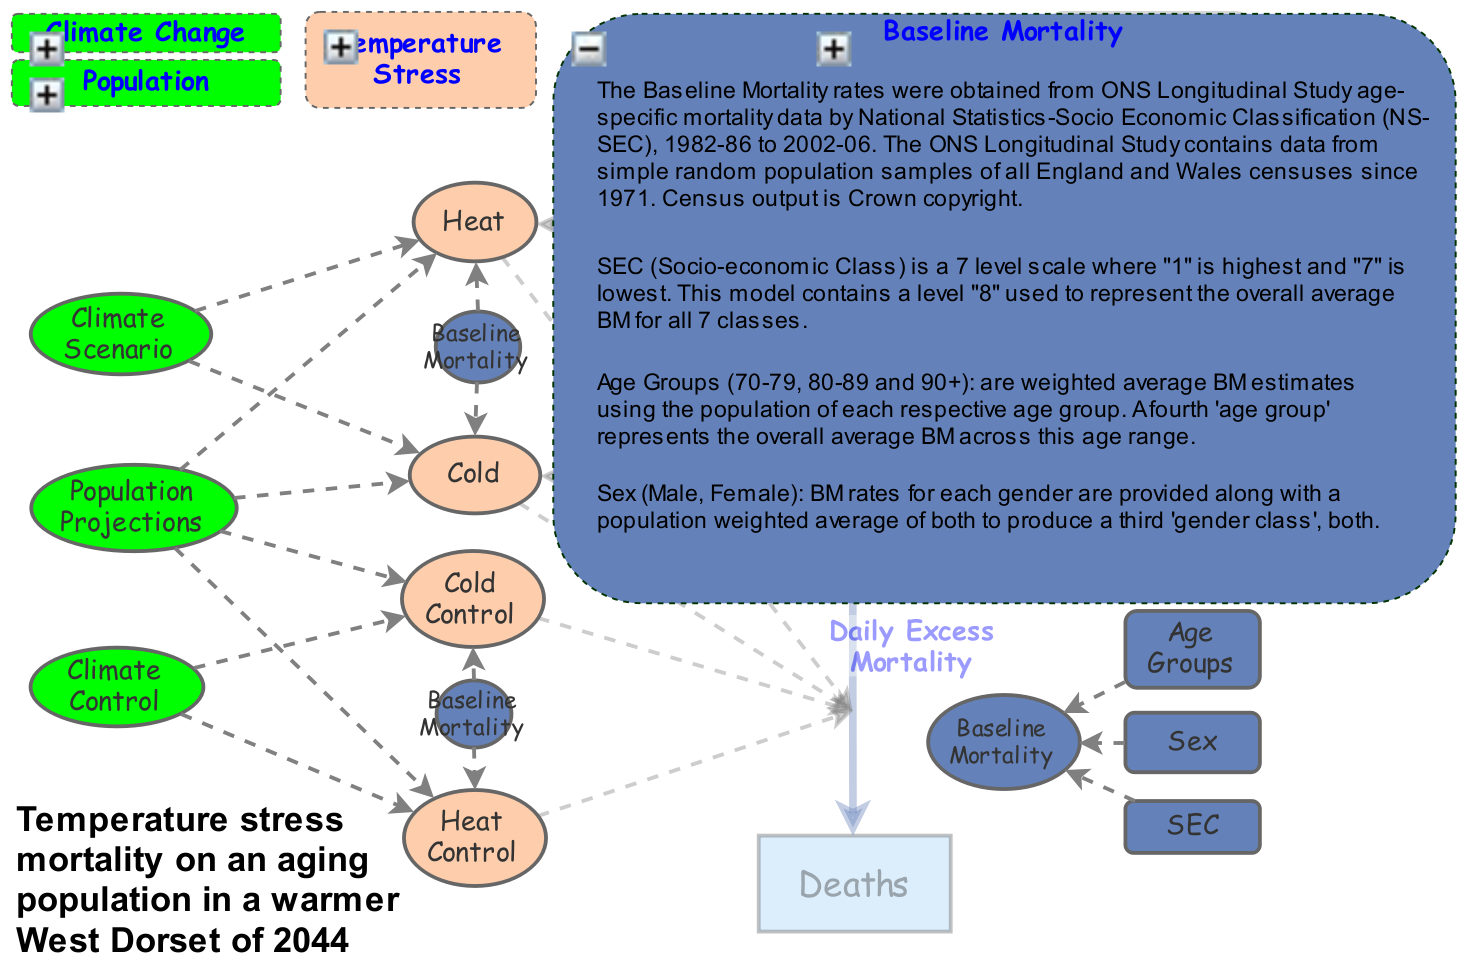
\includegraphics{./CCA/img/image_12.png}
	\caption[Population Variables]{This simulator allows the user to set the age group (4 groups for the over 70+ population are available), sex and socio-economic class (SEC 1-7 is from highest to lowest and 8 is for all classes).}
\end{figure}

\begin{figure}[htbp]
	\centering
	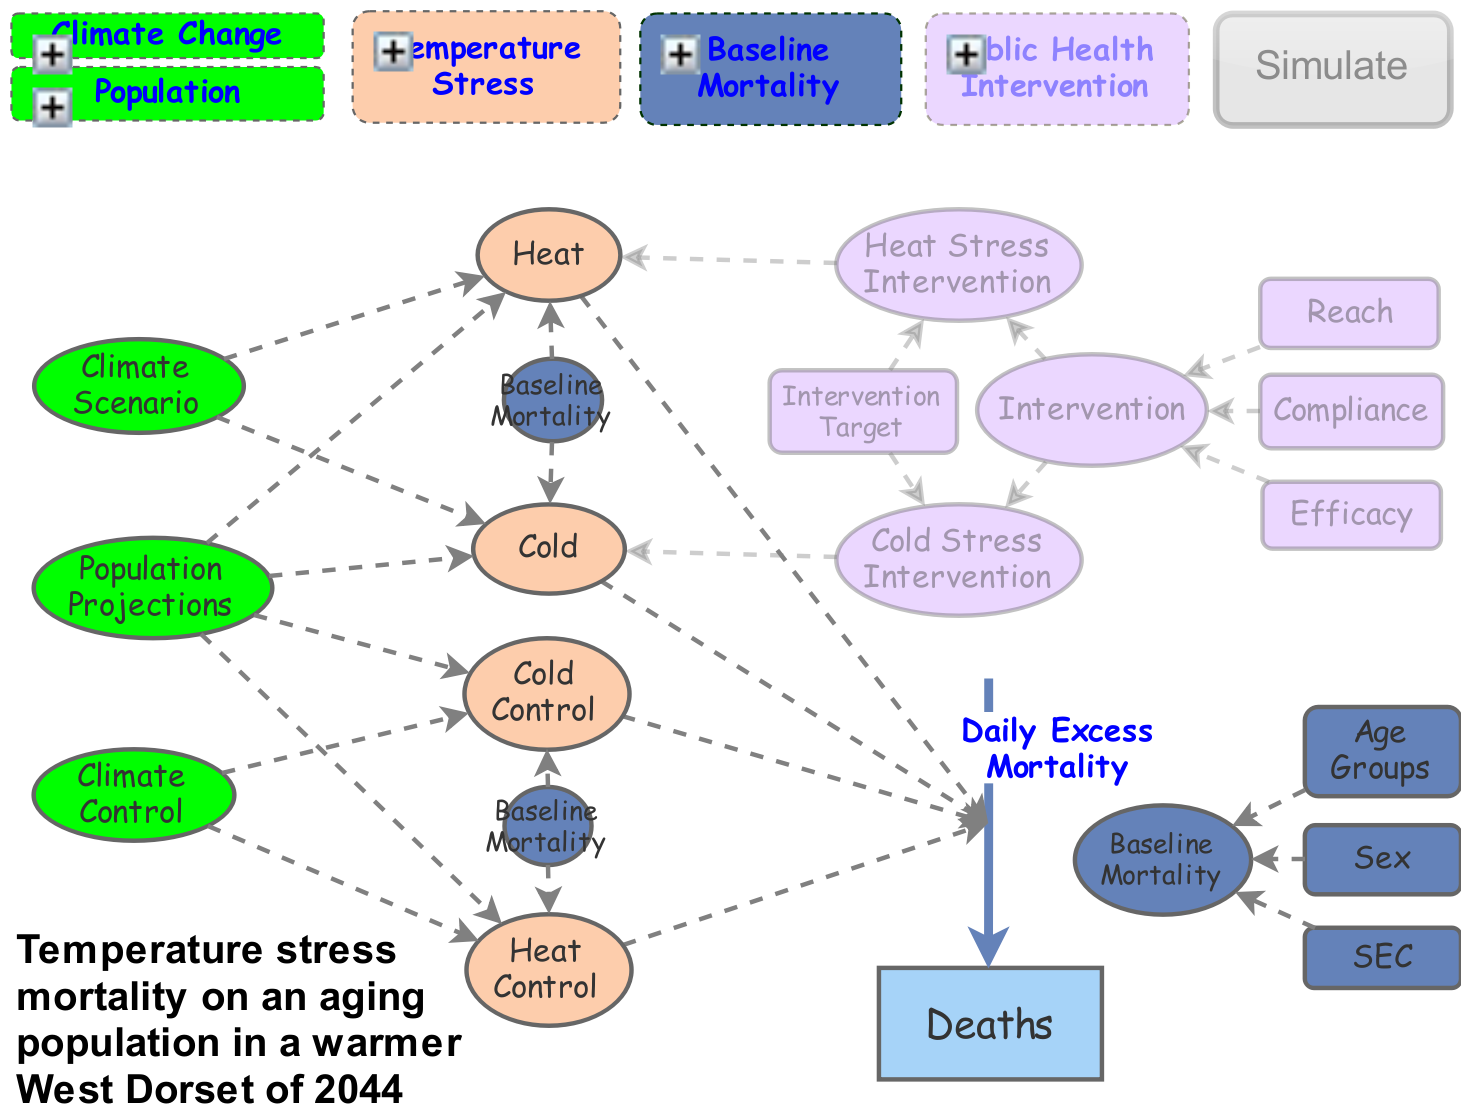
\includegraphics{./CCA/img/image_13.png}
	\caption[Cold Stress Excess Mortality is Higher]{It is worth noting at this point that even in a warmer West Dorset of 2044, mortality from cold stress will still be much higher than mortality from heat stress. Counter intuitive perhaps, but true. Of course excess mortality due to cold stress will be lower in the future (although still much higher than heat stress). More on this later -- it has implications for public health interventions. There are four `daily excess mortality' values estimated: excess mortality from future heat and cold stress and for comparison `control excess mortalities' are also estimated.}
\end{figure}

\begin{figure}[htbp]
	\centering
	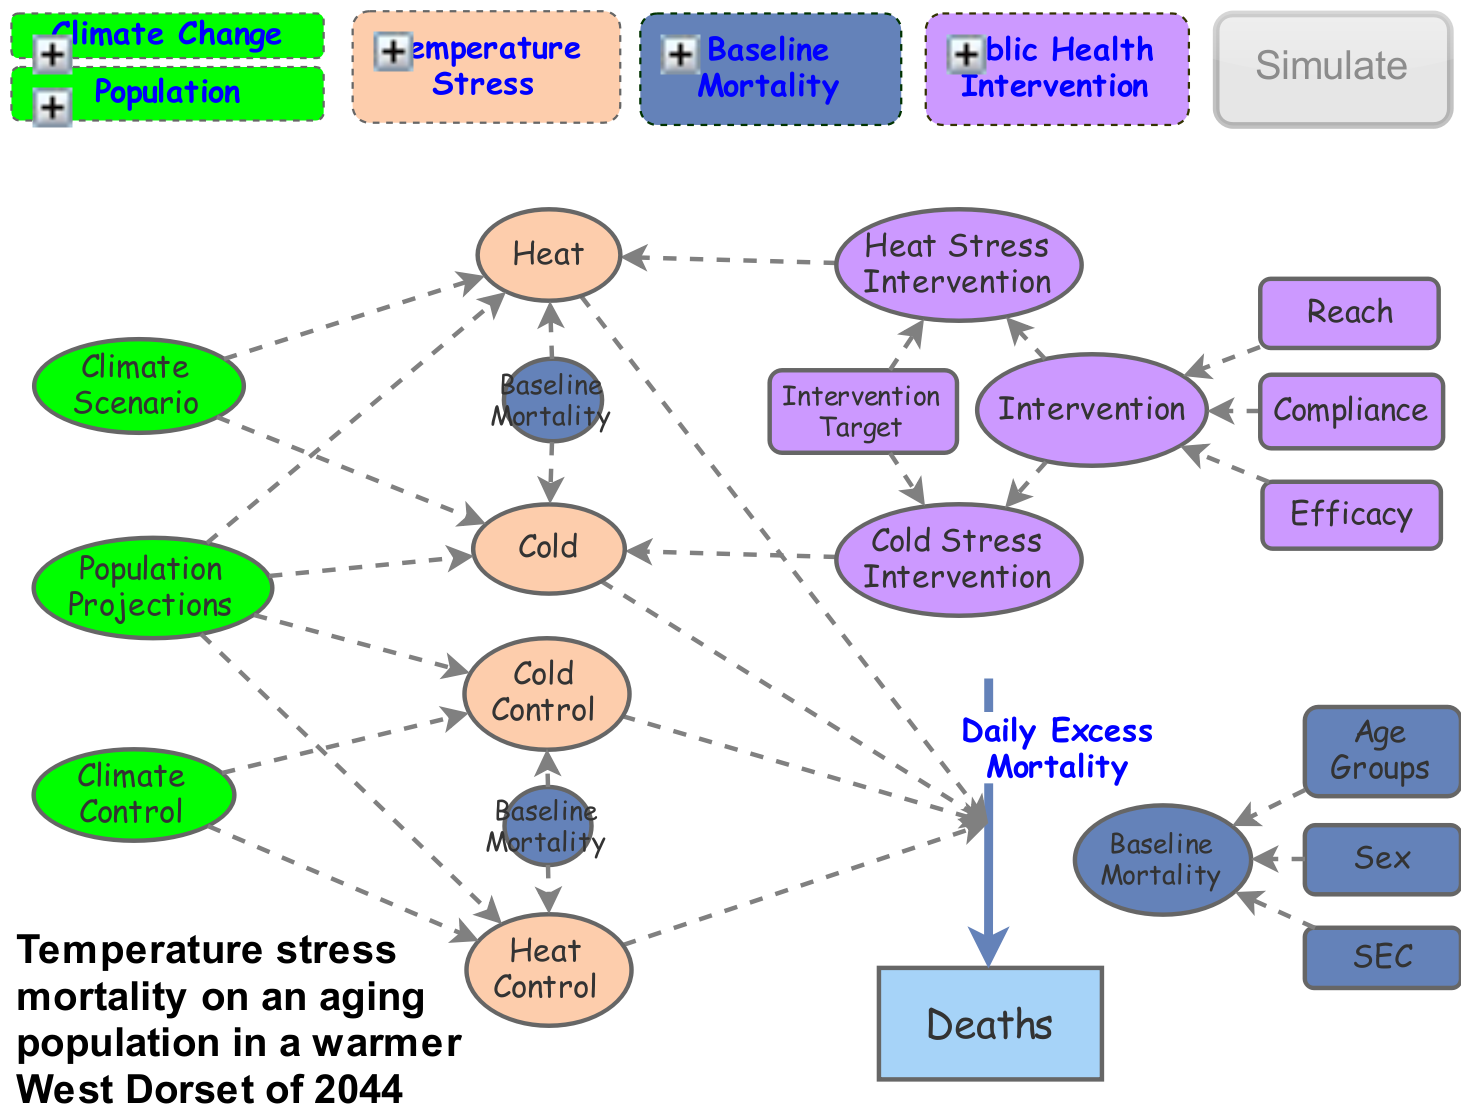
\includegraphics{./CCA/img/image_14.png}
	\caption[Devising Public Health Interventions]{You can compare these sources of excess mortality as they accumulate over the simulation period.So what public health interventions might be taken in order to assist the target population in adapting to more heat stress?}
\end{figure}

\begin{figure}[htbp]
	\centering
	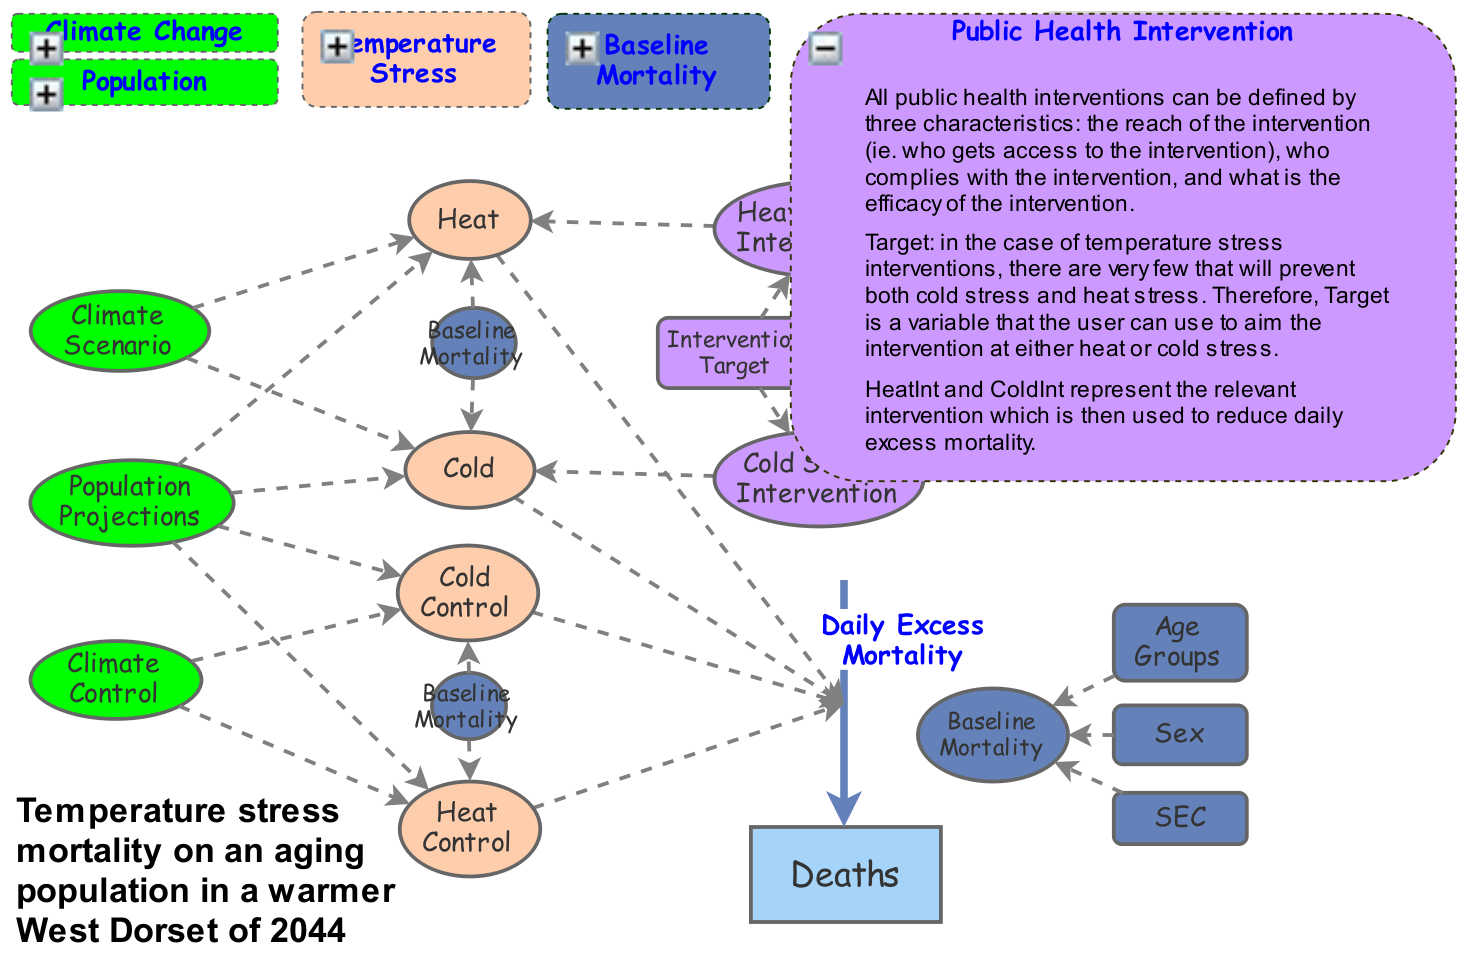
\includegraphics{./CCA/img/image_15.png}
	\caption[Intervention Targeting Options]{You have the option of trialling an intervention for either heat or cold stress, but not both at the same time. The default setting is for NO intervention. `Intervention Targeting' is the variable used to set which intervention will be made.}
\end{figure}

\begin{figure}[htbp]
	\centering
	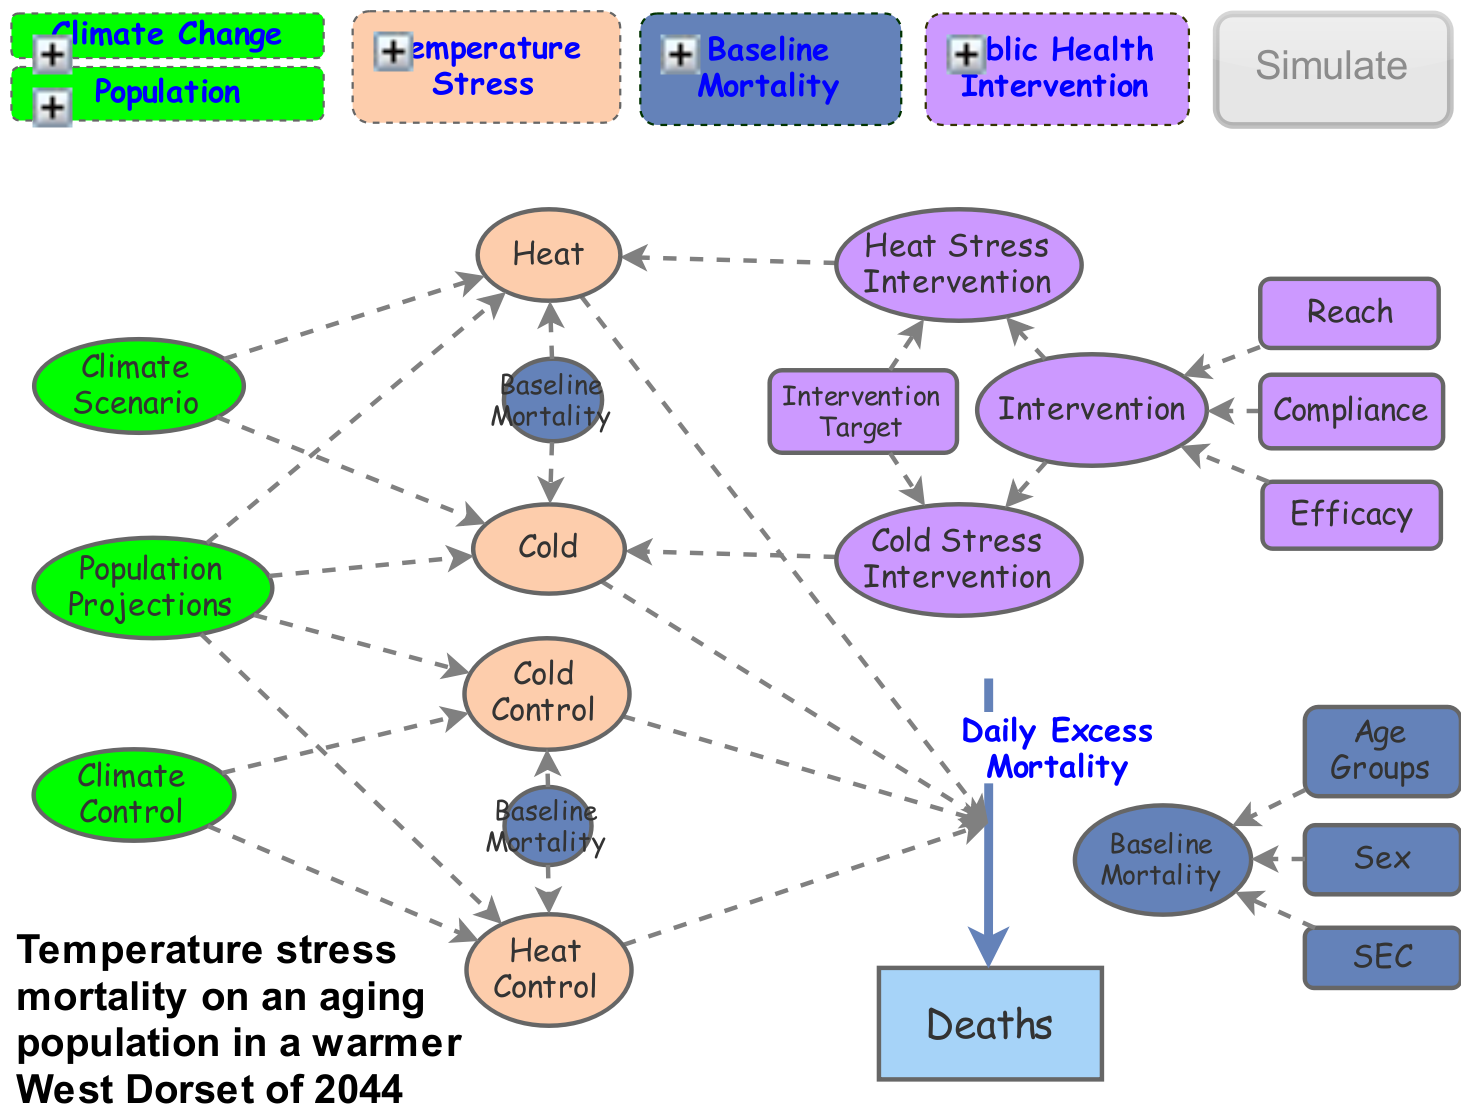
\includegraphics{./CCA/img/image_16.png}
	\caption[Elements of a Public Health Intervention]{All public health interventions have three basic variables: the proportion of the target population you can reach, the proportion of the population that comply with the intervention and the efficacy (how effective it is at doing what it is supposed to do) of the intervention.}
\end{figure}

\begin{figure}[htbp]
	\centering
	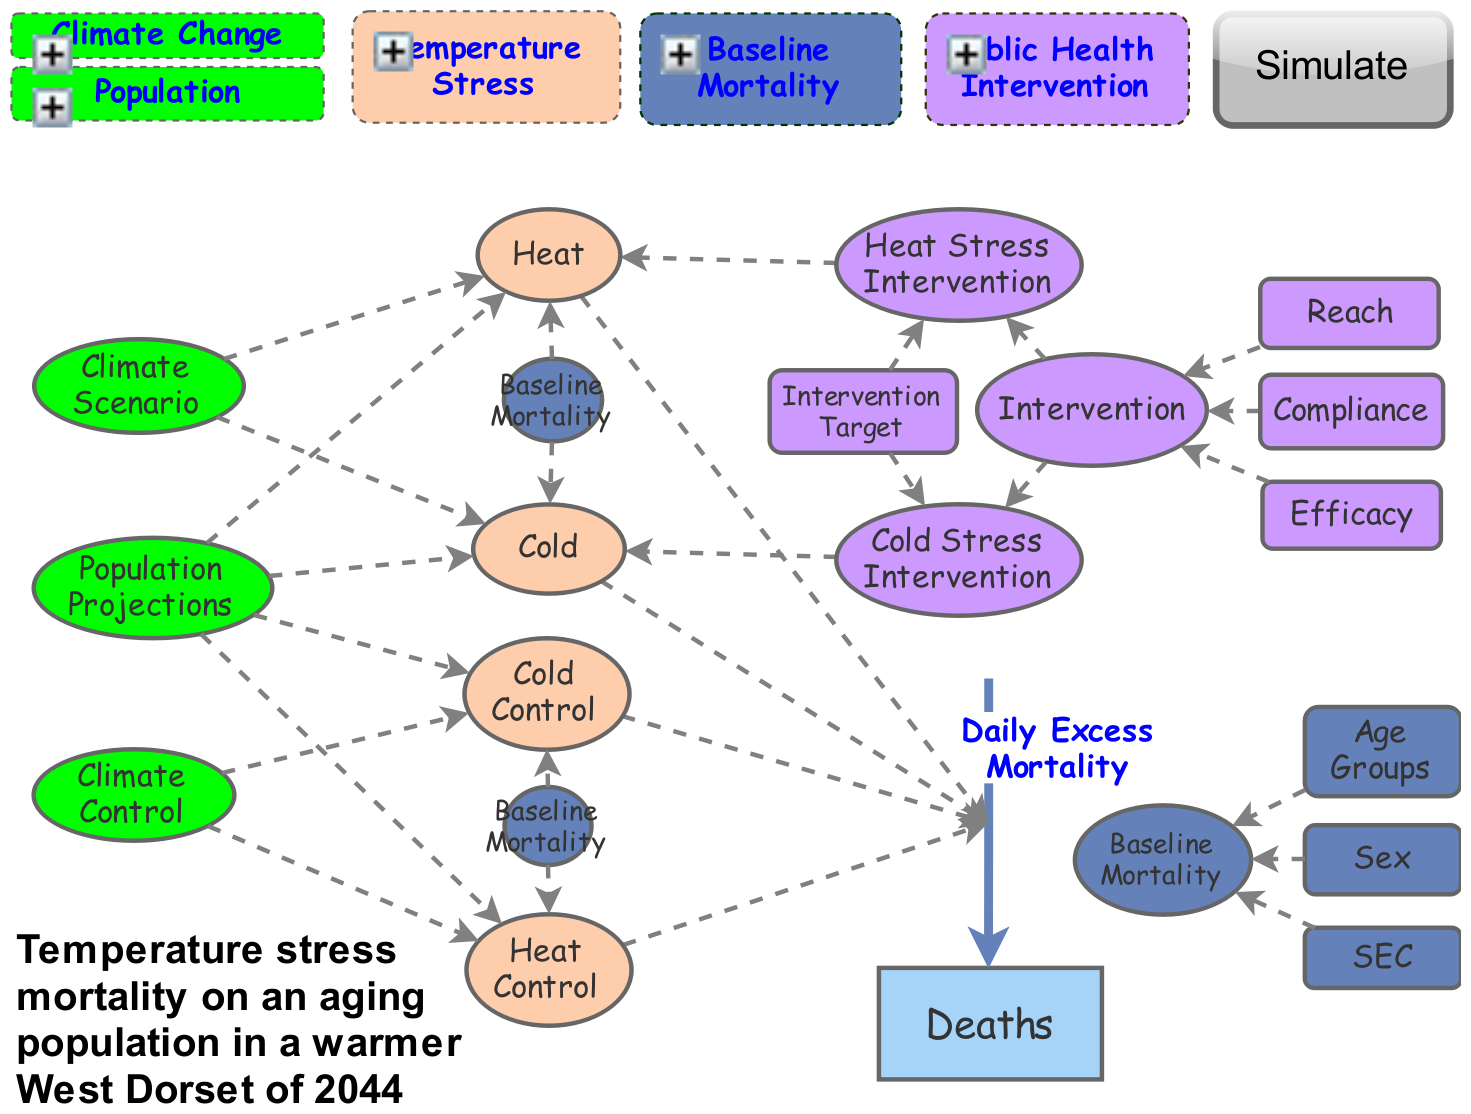
\includegraphics{./CCA/img/image_17.png}
	\caption[Run Simulation]{This `simulate' button produces the default simulation for a population with all age groups, all socio-economic classes and all both sexes included as a single population. Additionally, there are 10 years of simulated temperature data available (this default simulation setting uses the first 365 days). However, the `Settings' button at the top of the window allows the user to set the start and duration of the simulation period. The user will be presented with two daily excess mortality graphs (one for the future and one for the control), a combined accumulated deaths (both future and control) and a table of accumulated deaths.}
\end{figure}

\begin{figure}[htbp]
	\centering
	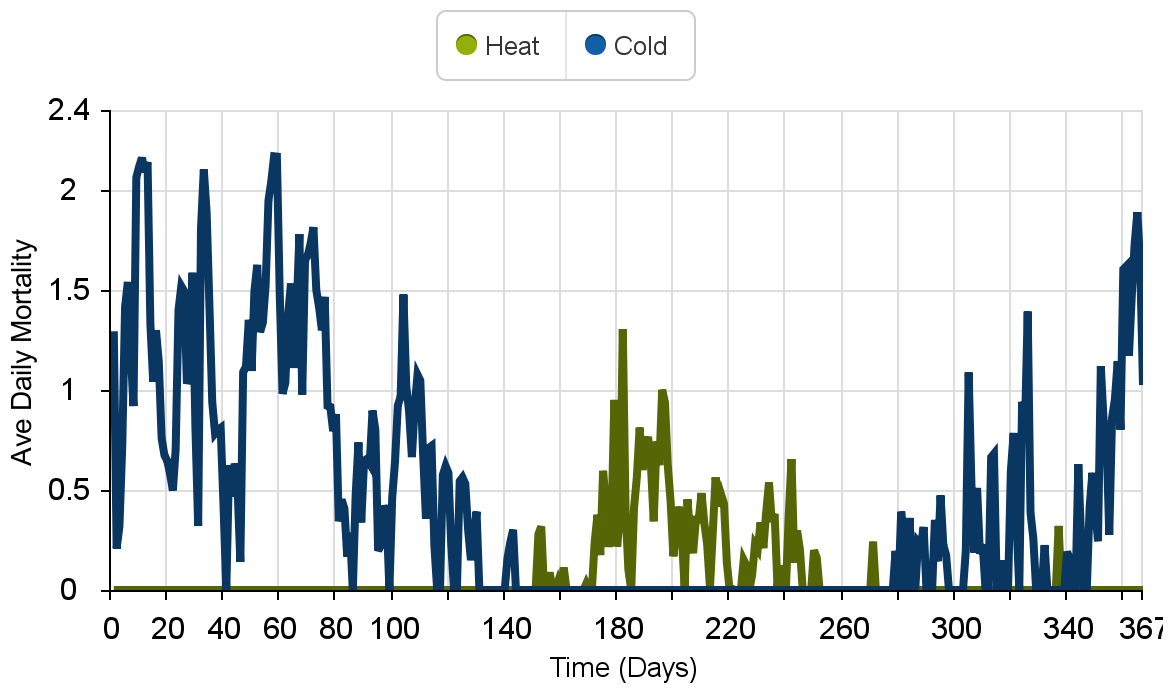
\includegraphics{./CCA/img/image_18.png}
	\caption[Simulation Output]{Do you see the three graph `tabs' above the graph? You can move between the visuals during the simulation. You can change the speed of the simulation and rerun it. The introduction to this model is now complete. You can `Exit Story' (bottom left of screen) and explore the model, its variables and its construction at your own pace. If you are unfamiliar with the Insight Maker modelling environment, you may wish to further explore that -- all models are open source -- set up your own free account to copy and modify this or any model for your own use and share with colleagues.}
\end{figure}
